\chapter{Prototype}

\begin{TempText}
	(Min 3, Max 5 pages)
\end{TempText}

\begin{TempText}
	@Note: The key goal of this part of the project is to develop a prototype of your game that distills out the core game play. The prototype should incorporate the game mechanics while providing only a crude approximation of other features like artwork.
\end{TempText}

% ====================================================================================

\section{Prototype Setup}

\begin{TempText}
	@Note: Include sketches and photos of your prototype in such a way that you can demonstrate how the prototype works and how the gameplay is modeled. How did you model environment, characters, and other features of the game?
\end{TempText}

We designed a playable paper prototype \ref{fig:prot_stalll} and \ref{fig:prot_0}.

\begin{figure}
    \centering
    \includegraphics[width=0.8\textwidth]{figures/Prototype/staaall.jpg}
    \caption{In the middle of a heated race.}
    \label{fig:prot_stalll}
\end{figure}

\begin{figure}
    \centering
    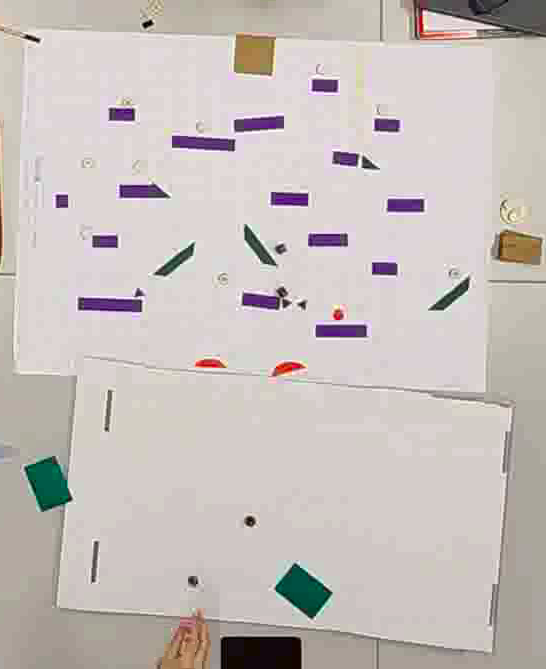
\includegraphics[width=0.8\textwidth]{figures/Prototype/vlcsnap-2022-03-20-18h52m10s352.png}
    \caption{Paper Prototype of the Game.}
    \label{fig:prot_0}
\end{figure}

Our design involves two types of people:
\begin{enumerate}
    \item Players: Play the game. Try to win by reaching the top first.
    \item Observer: Controls the automated game mechanics (such as the rising sand from the bottom) and makes sure the players abide by its rules.
\end{enumerate}

The players move on a grid plane. They take rounds, in each of which they can make a move. The raising sand from the bottom is modelled by a big piece of cardboard, which is moved 4 squares up every 2 rounds. If a player touches the rising sand, he dies.

On each round the players can move/jump to a new position.
There are two type of jump:
\begin{itemize}
    \item Easy Jump: A jump that does not go through falling sand and which finishes on a platform wider than 2 squares
    \item Hard Jump: A jump that goes through falling sand or which finishes on a platform narrower than 3 squares.
\end{itemize}

The players begin at the bottom of the level. Each player is represented by a differently coloured tetrahedron.

At every round, the players have 5 seconds to choose where they want to jump. They state their intended place of movement by putting a dice on their desired location. They can also state if they intend on using an action card. The list of action cards is shown at \ref{fig:prot_1} and \ref{fig:prot_2}.



\begin{figure}
    \centering
    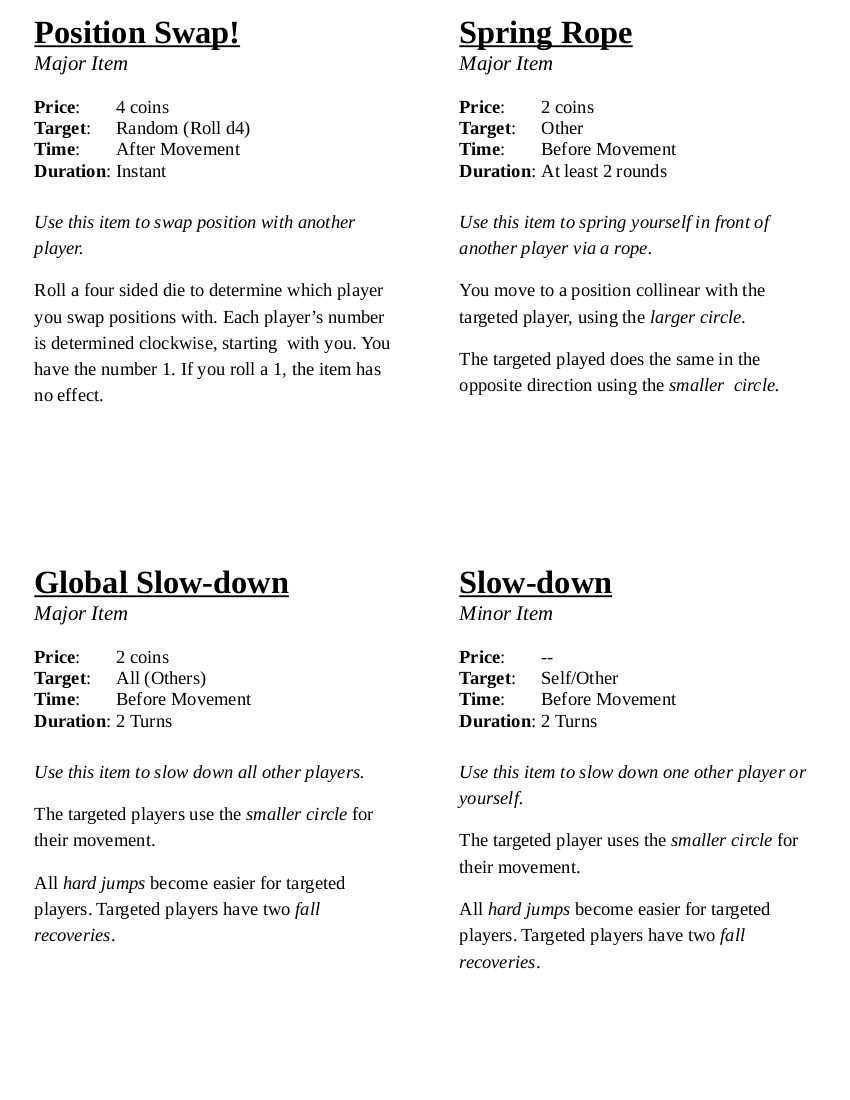
\includegraphics[width=0.8\textwidth]{figures/Prototype/topmeifyoucan_1.png}
    \caption{Action Cards.}
    \label{fig:prot_1}
\end{figure}



\begin{figure}
    \centering
    \includegraphics[width=0.8\textwidth]{figures/Prototype/topmeifyoucan_2.png}
    \caption{Action Cards.}
    \label{fig:prot_2}
\end{figure}


After the players finish making their choice, the Observer checks if all of the movements could be performed. This is done by picking up a circle, and checking if there is a position of the circle for which the beginning and ending positions of the players are  both points on the circle, and the arc of the circle do not go through any platforms. If this is the case, then the jump is possible. If the player performs a hard jump, he must say "even" or "odd" and then roll a dice. If he correctly calls the result, he successfully makes the jump. If he fails, then the player misses the platform and starts falling. For every platform he passes while falling, he has a chance of recovery. In order for him to recover, he must correctly call "odd" or "even" on a dice. If he calls correctly, then he makes a successful recovery and lands on the platform. Otherwise he continues falling. The falling stops when he reaches the bottom of the level, or when he hits the sand, which makes him die.

The game concludes when at least two of the players reach the top (represented by a brown square  at the top of the level).


\FloatBarrier


% ====================================================================================

\section{Playing Experience}

\begin{TempText}
	@Note: Your experience playing the game. Was it fun?
\end{TempText}

We played the game for more than two hours and find it to be quite fun. We found that it is very dependant on the rolling of the dice, and therefore on luck. This is a problem that will be less of an issue with the final product, as there this "luck" aspect will be replaced by the players' skill and ability to do good jumps.

% ====================================================================================

\section{Findings and Conclusion}

\begin{TempText}
	@Note: Explain what you have learned from creating the prototype. What has proved to be harder (or easier) than expected? What design revisions have you made to your game based on your experience creating the prototype?
\end{TempText}

\begin{itemize}
    \item We came to the conclusion that having a normal rope with which to tie two players is unnecessary. This is because it gives the players no clear advantage.

    This is the reason why the rope was modified to a "Spring Rope". Instead of tying two players together for a given set of rounds, the "Spring Rope" can be used by a player to quickly move in a given direction, similar to long jump. This makes the mechanics simpler and the item is more usable.
\end{itemize}



